\setbeamertemplate{section in toc}[sections numbered]

%% ====================== TITLE PAGE =====================
\titlegraphic{
    %\begin{block}{Auspician}
    
\includegraphics[width=0.22\textwidth]{Usach S2.png}
    \hspace{0.075\textwidth}
    
\includegraphics[width=0.25\textwidth]{usach_oocc/FASS.png}
    \hspace{0.075\textwidth}
    
\includegraphics[width=0.27\textwidth]{DIMEC-opc.2-color.png}
    %\end{block}
}

\begin{frame}[plain]
  \titlepage
\end{frame}

%% ====================== ÍNDICE =====================
\setbeamertemplate{navigation symbols}{}% hide nav symbols here
%\begin{frame}{Contenido}
%\begin{block}{Estructura de la presentación}
%\tableofcontents[hideallsubsections]
%\tableofcontents
%\end{block}
%\end{frame}

%% ====================== INTRODUCCIÓN =====================
\section{Introducción}
\begin{frame}{Contexto y motivación}
    \begin{itemize}
      \item La ventilación subterránea es crítica para la \textbf{seguridad y eficiencia} operativa en minería.\\[0.2cm]
      \item Los planes de mantenimiento tradicionales no siempre reflejan el \textbf{estado real de los ventiladores}.\\[0.2cm]
      \item Se plantea \textbf{correlacionar mediciones experimentales con simulaciones CFD} para habilitar \textbf{mantenimiento predictivo}.
    \end{itemize}
\end{frame}

%% ====================== OBJETIVOS =====================
\begin{frame}{Objetivo general}
    \centering
    \begin{block}{}
    \begin{quote}    
    Diseñar e implementar un \textcolor{UsachVerde}{modelo a escala de un túnel de viento} con analogía a sistemas de ventilación minera, con \textcolor{UsachVerde}{instrumentación y control basados en Arduino}, a fin de evaluar y correlacionar datos de operación con un modelo de \textcolor{UsachVerde}{Dinámica de Fluidos Computacional (CFD)} para el desarrollo de estrategias de \textcolor{UsachVerde}{mantenimiento predictivo}.
    \end{quote}
    \end{block}
\end{frame}

\begin{frame}{Objetivos específicos}
    \begin{enumerate}
      \item Construir el prototipo e integrar la instrumentación.\\[-0.2cm]
      \item Desarrollar y calibrar el modelo CFD.\\[-0.2cm]
      \item Comparar resultados simulados con datos experimentales.\\[-0.2cm]
      \item Proponer lineamientos de mantenimiento predictivo.
    \end{enumerate}
\end{frame}

%% ====================== METODOLOGÍA =====================
\section{Metodología}
\begin{frame}{Flujo de trabajo general}
    \centering
    \begin{enumerate}
        \item Diseño y construcción del túnel de viento.
        \item Instrumentación (corriente, voltaje, temperatura, vibración, flujo).
        \item Diseño de interfaz de control y manejo de datos.
        \item Modelo CFD en \textit{ANSYS Fluent}.
        \item Validación y ajuste.
        \item Lineamientos mantenimiento predictivo.
    \end{enumerate}
\end{frame}

\subsection{Prototipo experimental}
\begin{frame}{Túnel de viento a escala}
    \begin{columns}
        \column{0.6\textwidth}
        \centering
        
\includegraphics[height=0.1\textwidth]{dump/inventor.png}
        \\[0.5cm]
        \begin{itemize}
          \item Ventilador axial 120~mm regulado por PWM (0--4500 RPM).
          \item Sección circular de 94mm de diámetro y 480mm de largo.
          \item Diseño de cámara suspendida mediante resortes.
        \end{itemize}
        \column{0.4\textwidth}
            \begin{block}{}
            \begin{figure}[ht!]
                \centering
                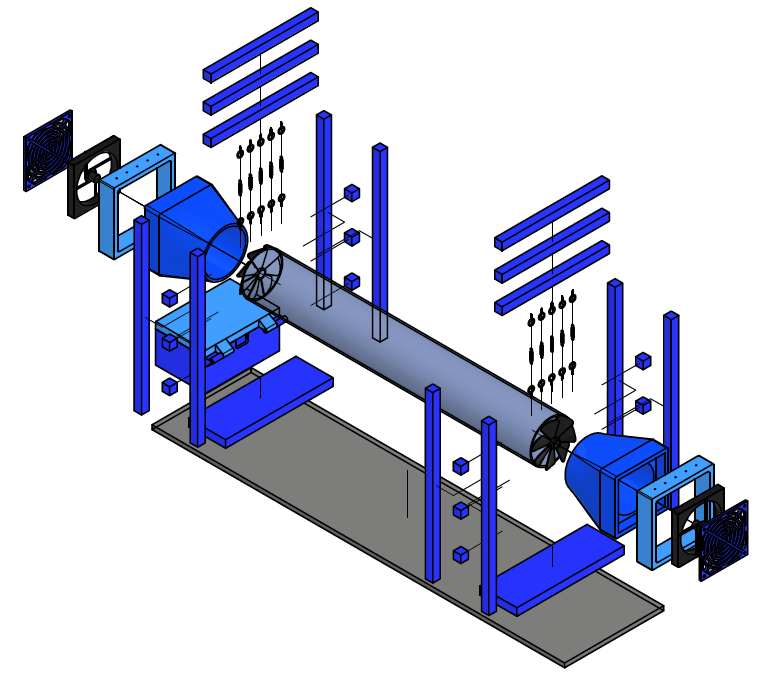
\includegraphics[width=\textwidth]{dump/explo.png}
                \caption{Vista explosionada del modela CAD del dispositivo experimental.}
            \end{figure}
            \end{block}
    \end{columns}
\end{frame}

\begin{frame}{Instrumentación}
    \begin{columns}
        \column{0.5\textwidth}
        \begin{block}{}
            \begin{figure}[ht!]
                \centering
                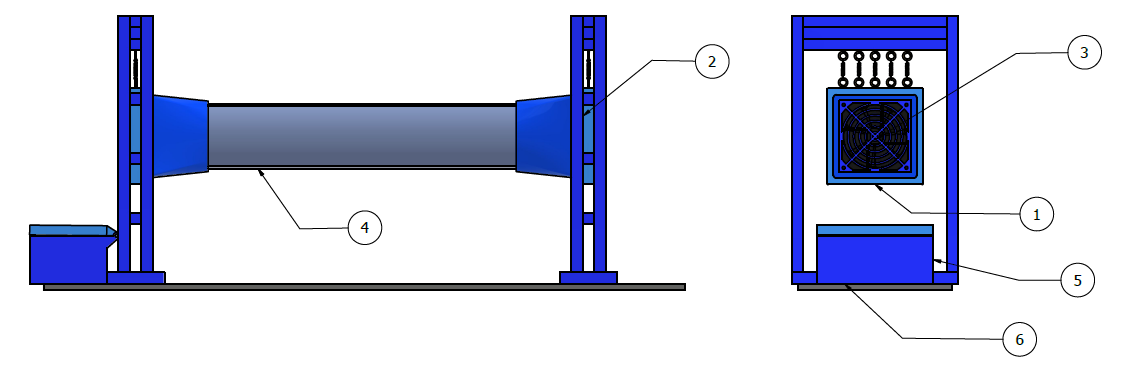
\includegraphics[width=\textwidth]{dump/sens.png}
                \caption{Esquema de disposición de los sensores.}
            \end{figure}
            \end{block}
        \begin{block}{Parámetros monitorizados}
          Corriente, voltaje, temperatura del motor, vibración radial, velocidad del flujo de aire.
        \end{block}
        \column{0.5\textwidth}
        \begin{enumerate}
            \item Sensor de Corriente ACS712.
            \item Sensor de Voltaje PWM (0-25 V).
            \item Sensor de Temperatura LM35.
            \item Cámara Térmica AMG8833.
            \item Acelerómetro MPU6050.
            \item Sensor de Flujo de Aire Indirecto (Anemómetro Calibrado).
        \end{enumerate}
        Los sensores se conectan a una placa de desarrollo ESP32.
    \end{columns}
\end{frame}

\begin{frame}{Obtención de datos}
\begin{columns}
    \column{0.5\textwidth}
    \begin{itemize}
        \item Microcontrolador Arduino con servicio REST API.
        \item Control de velocidad del ventilador y muestreo de datos.
        \item Datos graficados en vivo y almacenados en la base de datos.
    \end{itemize}
    \centering
    \\[1cm]
    
\includegraphics[height=0.13\textwidth]{dump/arduino.png}
    \hspace{0.1cm}
    
\includegraphics[height=0.13\textwidth]{dump/node.png}
    \hspace{0.1cm}
    
\includegraphics[height=0.13\textwidth]{dump/sql.png}
    \column{0.5\textwidth}
    \begin{block}{}
            \begin{figure}[ht!]
                \centering
                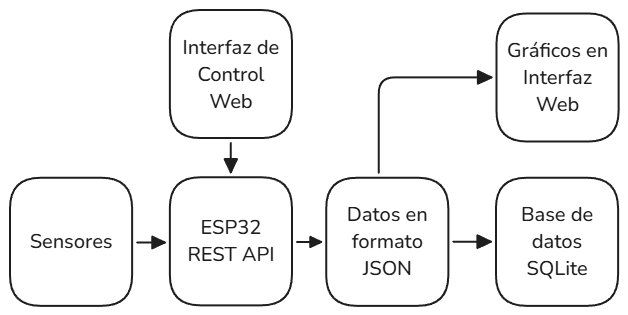
\includegraphics[width=\textwidth]{dump/diaaaa.png}
                \caption{Esquema de obtención de datos.}
            \end{figure}
            \end{block}
\end{columns}
\end{frame}

\begin{frame}{Interfaz de control}
    \begin{columns}
    \column{0.5\textwidth}
    \centering
        \begin{block}{}
            \begin{figure}[ht!]
                \centering
                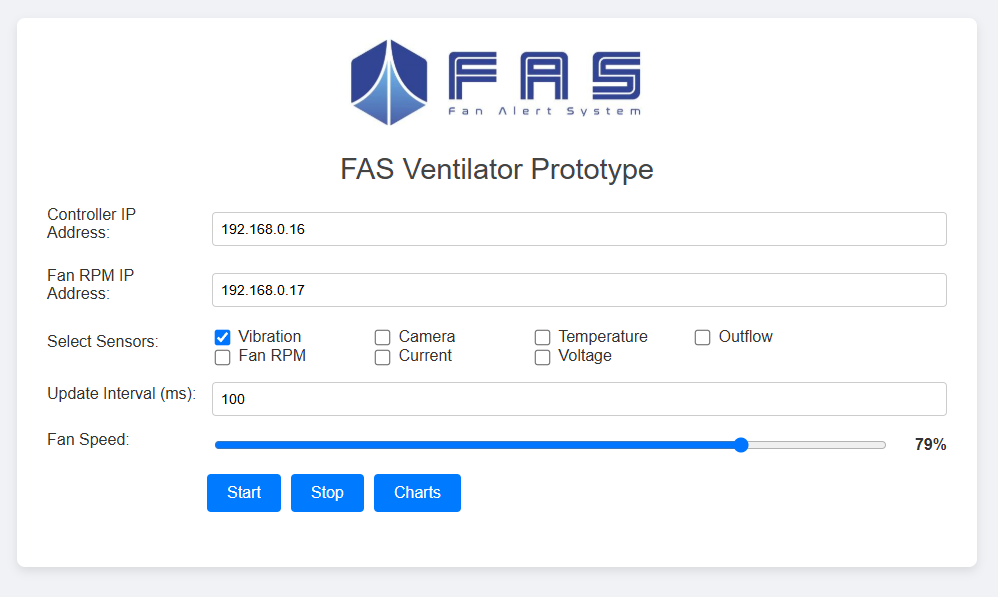
\includegraphics[width=\textwidth]{dump/web.png}
                \caption{Panel de control del dispositivo experimental.}
            \end{figure}
        \end{block}
            
\includegraphics[height=0.14\textwidth]{dump/stack.png}
    \column{0.5\textwidth}
        \begin{itemize}
            \item Permite el control y monitoreo del dispositivo.
            \item Almacena los datos de sensores y condiciones de operación.
        \end{itemize}
        \begin{block}{}
            \begin{figure}[ht!]
                \centering
                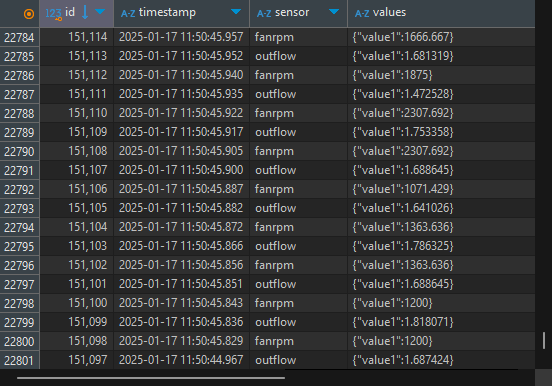
\includegraphics[width=0.6\textwidth]{dump/table.png}
                \caption{Ejemplo de tabla de datos de sensores.}
            \end{figure}
        \end{block}       
    \end{columns}
\end{frame}

\subsection{Modelo CFD}
\begin{frame}{Preparación del Modelo CAD}
\begin{columns}
\column{0.5\textwidth}
\centering

\includegraphics[height=0.3\textwidth]{dump/Spaceclaim.png}
\begin{itemize}
    \item Modelo simplificado del volúmen de control con regiones delimitadas.
\end{itemize}
\column{0.5\textwidth}
        \begin{block}{}
            \begin{figure}[ht!]
                \centering
                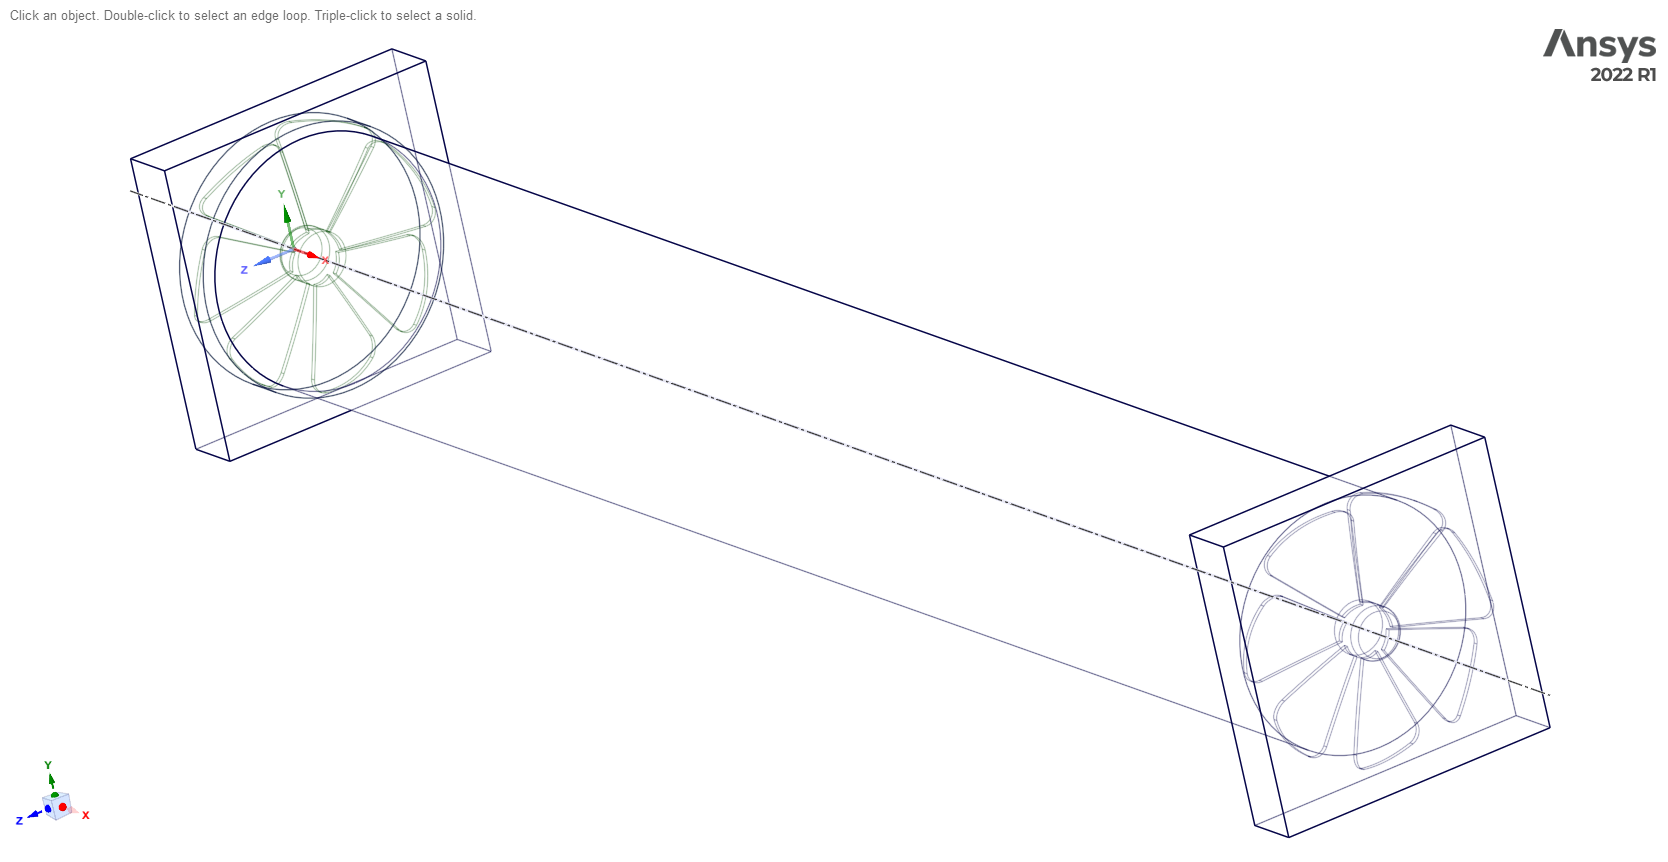
\includegraphics[width=\textwidth]{dump/space.png}
                \caption{Geometría del modelo en ANSYS SpaceClaim.}
            \end{figure}
        \end{block}  
\end{columns}
\end{frame}

\begin{frame}{Mallado del modelo}
    \begin{columns}
        \column{0.4\textwidth}
        \centering
        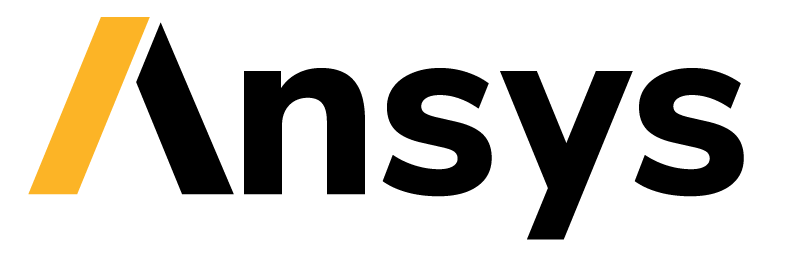
\includegraphics[height=0.13\textwidth]{dump/ansys.png}
        \\[0.5cm]
            \begin{itemize}
                \item Malla de hexahedros y tetraedros.
                \item Refinamiento por zonas.
            \end{itemize}
        \column{0.6\textwidth}
        \begin{block}{}
            \begin{figure}[ht!]
                \centering
                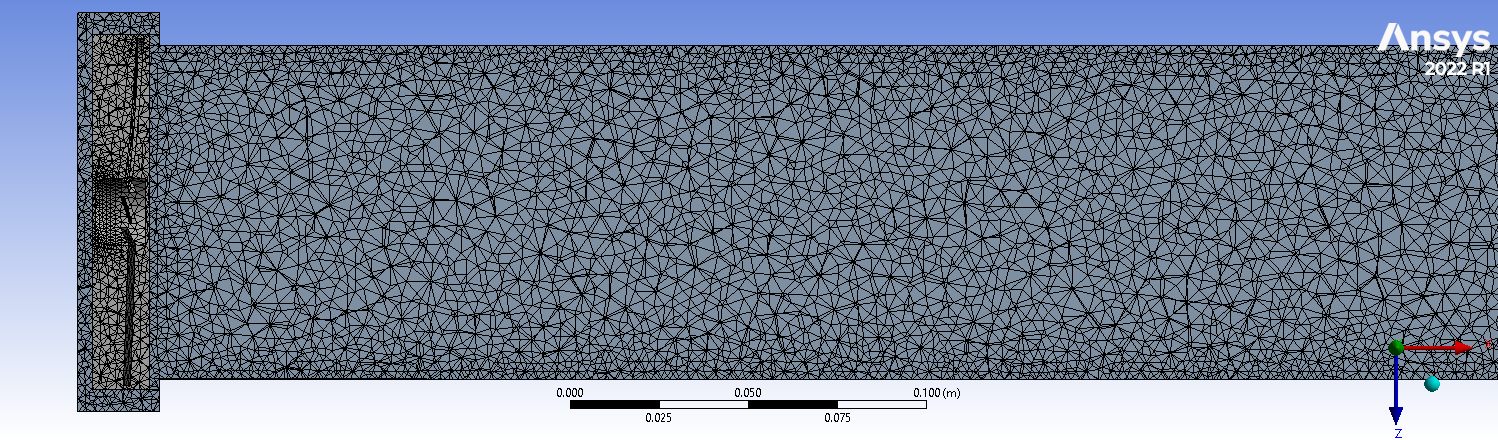
\includegraphics[width=\textwidth]{dump/mesh.png}
                \caption{Mallado realizado en ANSYS Mesher.}
            \end{figure}
        \end{block}  
    \end{columns}
\end{frame}

\begin{frame}{Configuración del modelo CFD}
    \begin{columns}
        \column{0.5\textwidth}
        \centering
        
\includegraphics[height=0.3\textwidth]{dump/fluent.png}
    \begin{itemize}
        \item Algorítmo SIMPLE para flujo incompresible.
        \item Modelo de turbulencia $k-\epsilon$.
        \item Condiciones de contorno de entradas o salida de presión.
        \item Velocidades fijas de rotación del ventilador.
        \item Aire como fluido ideal:
        \begin{itemize}
            \item Densidad $1.225 kg/m^3$
            \item Viscosidad de $1.8\cdot 10^{-5} Pa\cdot s$
        \end{itemize}
    \end{itemize}
    \column{0.5\textwidth}
    \begin{block}{}
            \begin{figure}[ht!]
                \centering
                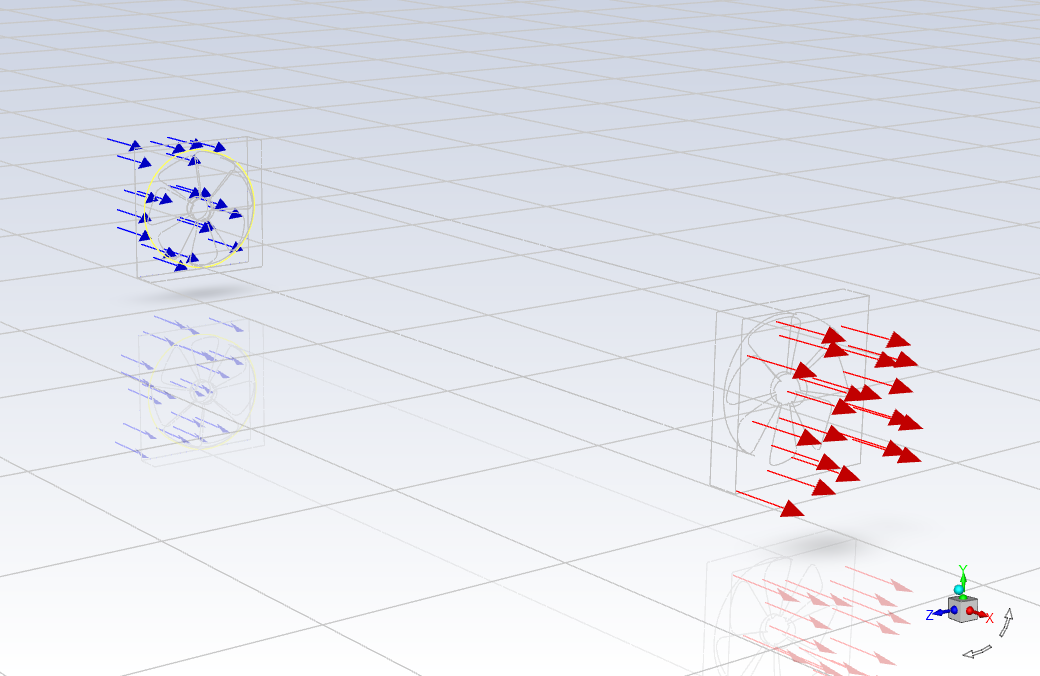
\includegraphics[width=\textwidth]{dump/borde.png}
                \caption{Condiciones de borde aplicadas en ANSYS Fluent.}
            \end{figure}
        \end{block}  
    \end{columns}
\end{frame}

\subsection{Validación}
\begin{frame}{Estrategia de validación}
\begin{columns}
\column{0.7\textwidth}
\begin{enumerate}
  \item Ejecutar simulaciones estacionarias a 833, 2500 y 4200 RPM.
  \item Medir velocidad media a la salida del dispositivo.
  \item Calcular error porcentual relativo $\epsilon$.
\end{enumerate}
\vspace{0.3cm}
Se evalúa el error promedio y la correlación entre el modelo CFD y el modelo experimental construído.
\column{0.3\textwidth}
\begin{block}{Error porcentual relativo}
    \(\varepsilon = \frac{|U_{exp}-U_{sim}|}{U_{exp}}\times100\%\)
\end{block}
\end{columns}
\end{frame}

%% ====================== RESULTADOS =====================
\section{Resultados}
\begin{frame}{Comparación velocidad del flujo}
\begin{columns}
    \column{0.55\textwidth}
\begin{table}
\begin{block}
\centering
\begin{tabular}{@{}lccc@{}}
  \toprule
  \textbf{RPM} & \textbf{$U_{exp}$ (m/s)} & \textbf{$U_{sim}$ (m/s)} & \textbf{Error (\%)} \\
  \midrule
  833  & 0.63 & 0.46 & 26.98 \\
  2500 & 1.80 & 1.34 & 25.56 \\
  4200 & 2.75 & 2.12 & 22.91 \\
  \bottomrule
\end{tabular}
  \caption{Comparación de velocidades promedio medidas y simuladas a diferentes RPM del ventilador.}
\end{block}
  \end{table}
\end{columns}
\end{frame}

\begin{frame}{Cálculo y convergencia}
    \begin{columns}
        \column{0.5\textwidth}
        \begin{block}{}
        \begin{figure}[ht!]
            \centering
            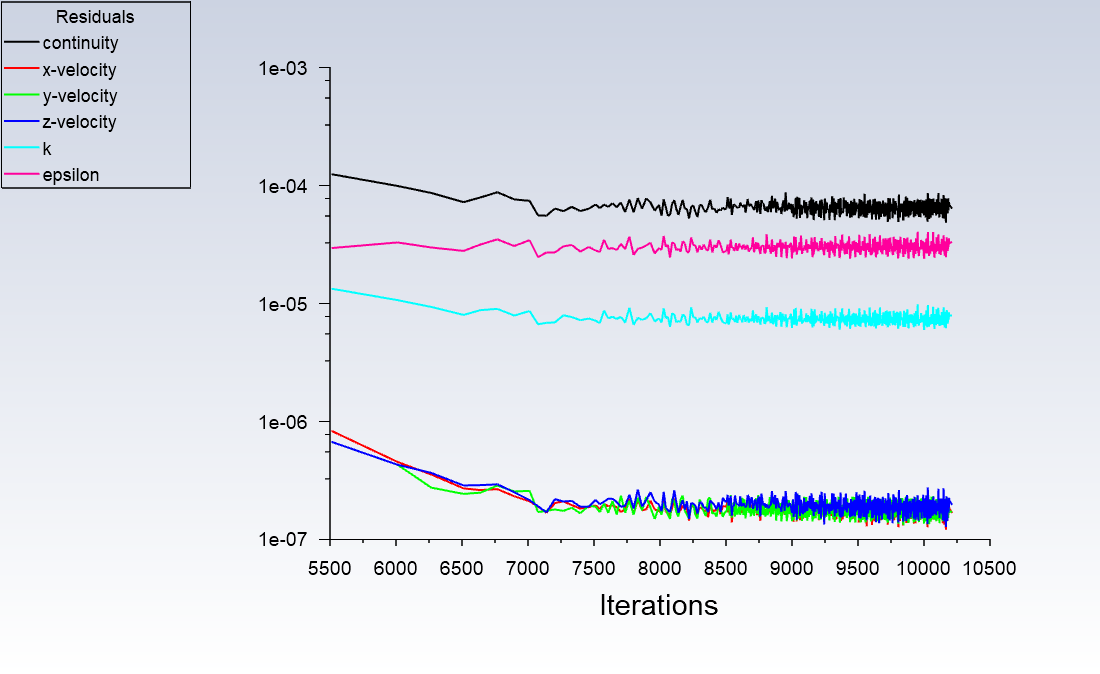
\includegraphics[width=\linewidth]{dump/res1.png}
            \caption{Gráfico de convergencia para 833 RPM.}
        \end{figure}
    \end{block}
    \column{0.5\textwidth}
    \begin{block}{}
        \begin{figure}[ht!]
            \centering
            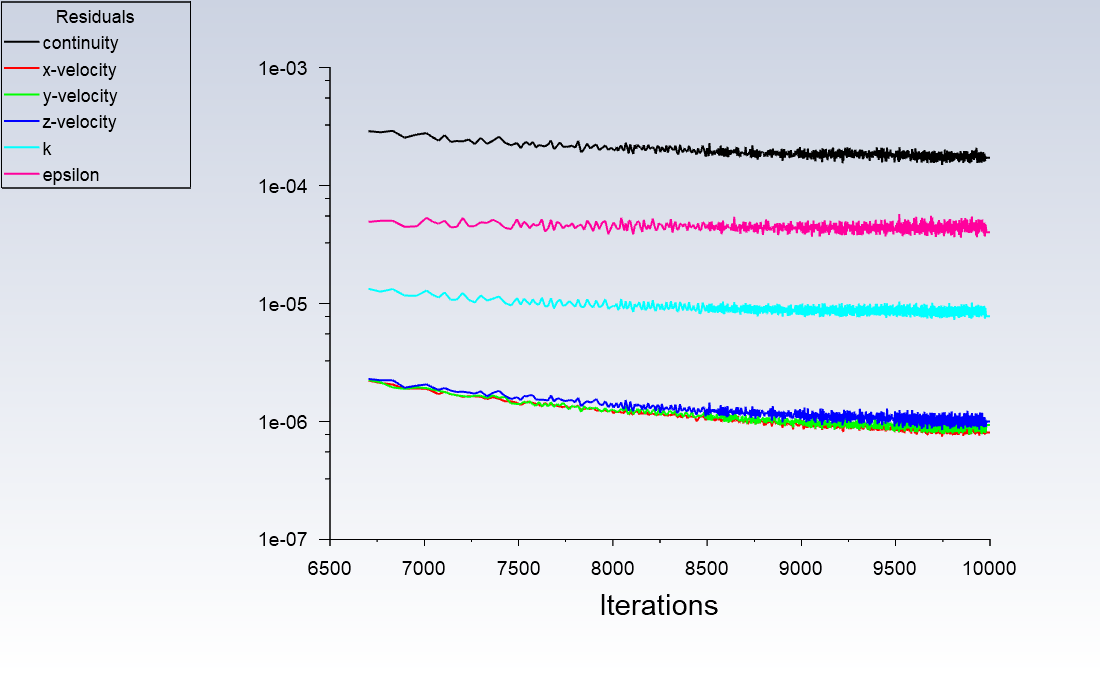
\includegraphics[width=\linewidth]{dump/res3.png}
            \caption{Gráfico de convergencia para 4200 RPM.}
        \end{figure}
    \end{block}
    \end{columns}
\end{frame}

\begin{frame}{Distribución de velocidades (4200 RPM)}
    \begin{block}{}
        \begin{figure}[ht!]
            \centering
            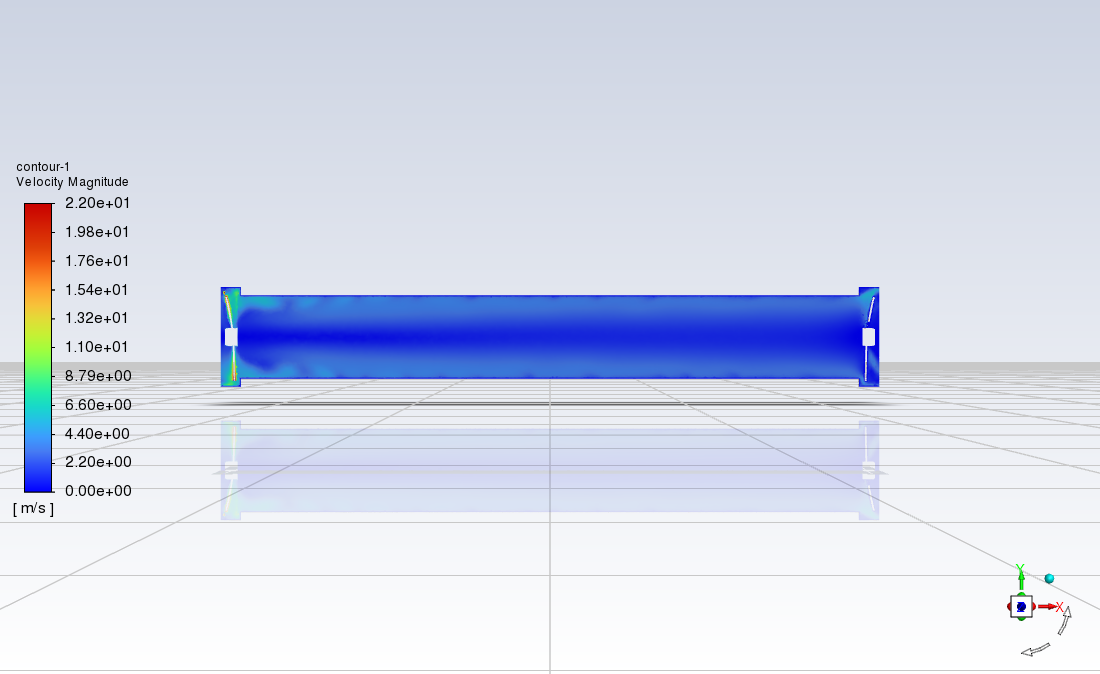
\includegraphics[width=0.6\linewidth]{dump/vel3.png}
            \caption{Contornos de velocidad simulados (m/s) en el plano central del túnel para 4200 RPM.}
        \end{figure}
    \end{block}
\end{frame}

\begin{frame}{Presiones estáticas y dinámicas}
    \begin{columns}
        \column{0.5\textwidth}
        \begin{block}{}
        \begin{figure}[ht!]
            \centering
            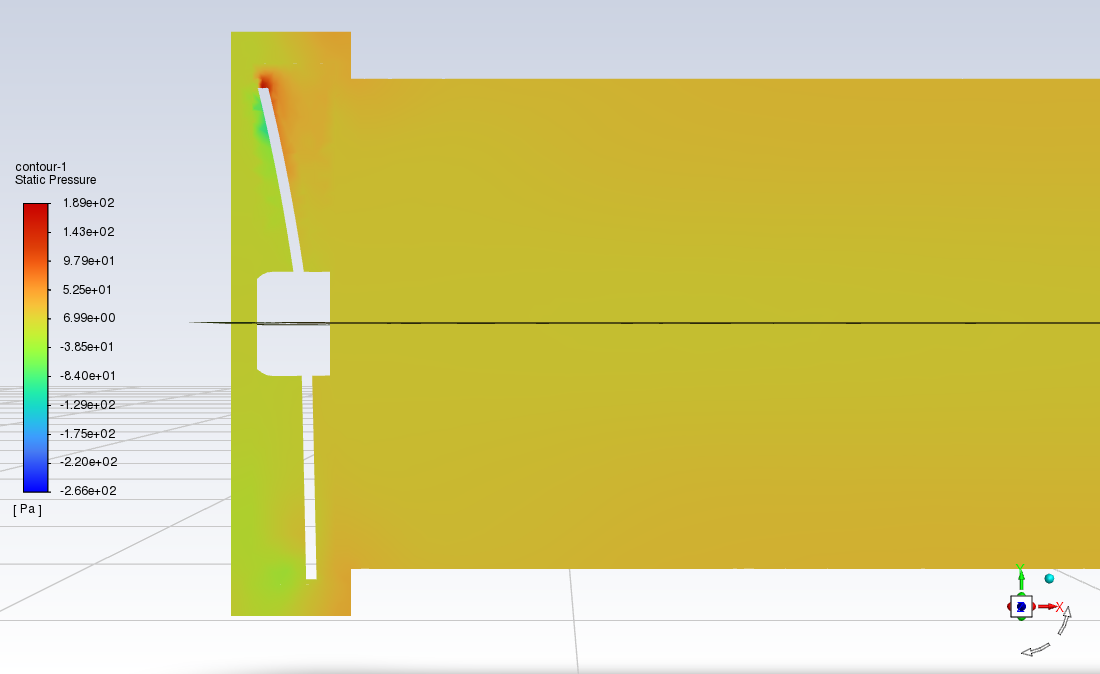
\includegraphics[width=\linewidth]{dump/sta3.png}
            \caption{Presión estática para 4200 RPM.}
        \end{figure}
    \end{block}
    \column{0.5\textwidth}
    \begin{block}{}
        \begin{figure}[ht!]
            \centering
            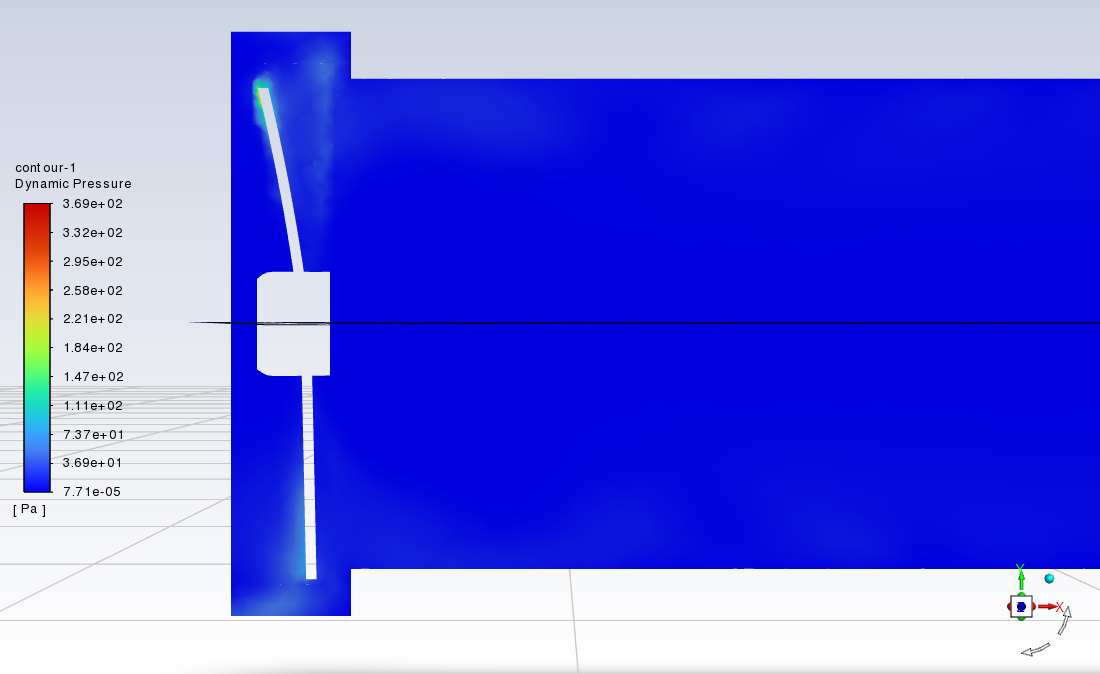
\includegraphics[width=\linewidth]{dump/dyn3.png}
            \caption{Mapa de presión dinámica para 4200 RPM.}
        \end{figure}
    \end{block}
    \end{columns}
\end{frame}

\begin{frame}{Lineas de corrientes}
    \begin{columns}
        \column{0.33\textwidth}
        \begin{block}{}
        \begin{figure}[ht!]
            \centering
            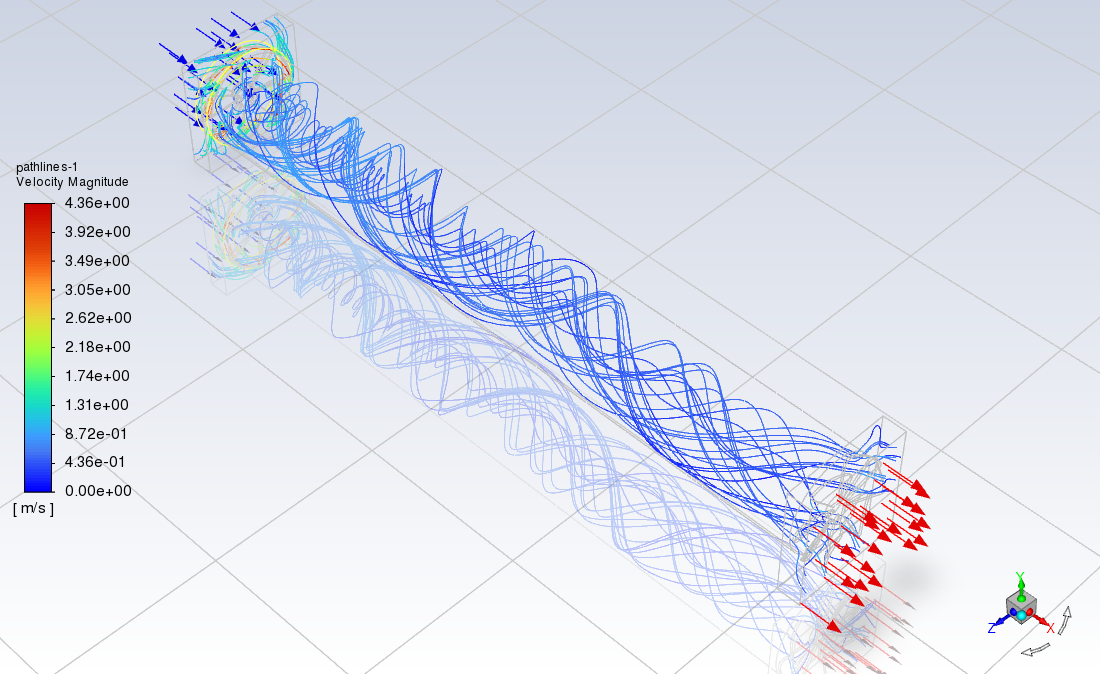
\includegraphics[width=\linewidth]{dump/cor1.png}
            \caption{Líneas de corrientes para 833 RPM.}
        \end{figure}
    \end{block}
    \column{0.33\textwidth}
        \begin{block}{}
        \begin{figure}[ht!]
            \centering
            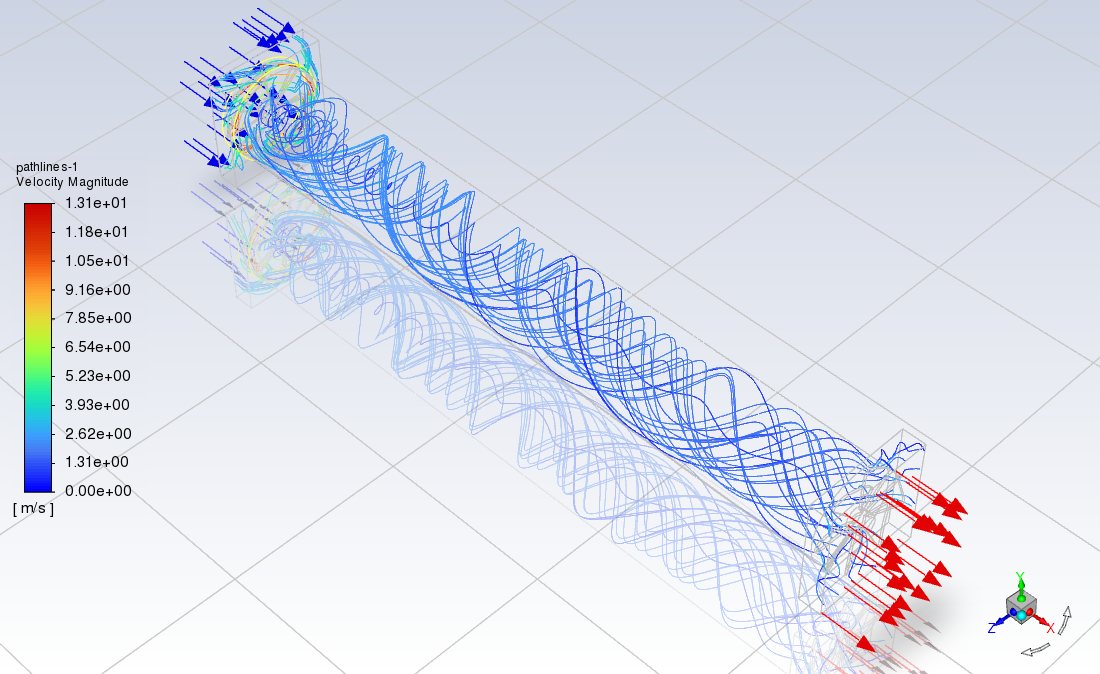
\includegraphics[width=\linewidth]{dump/cor2.png}
            \caption{Líneas de corrientes para 2500 RPM.}
        \end{figure}
    \end{block}
    \column{0.33\textwidth}
        \begin{block}{}
        \begin{figure}[ht!]
            \centering
            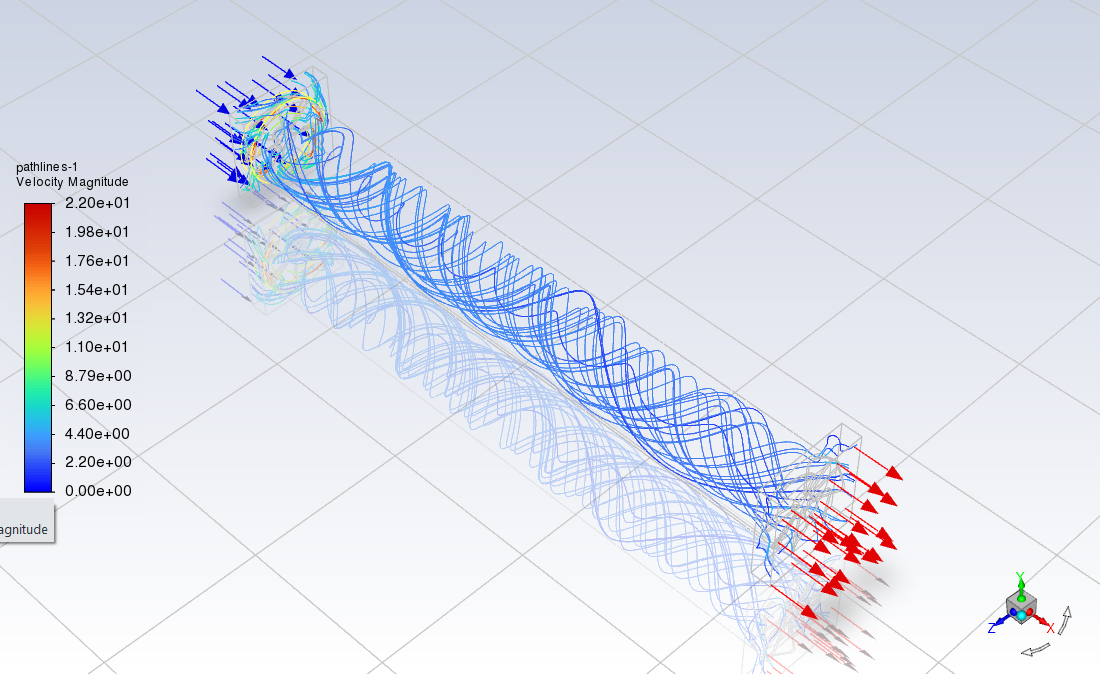
\includegraphics[width=\linewidth]{dump/cor3.png}
            \caption{Líneas de corrientes para 4200 RPM.}
        \end{figure}
    \end{block}
    \end{columns}
\end{frame}

\begin{frame}{Mapa de velocidad en salida (4200 RPM)}
    \begin{block}{}
        \begin{figure}[ht!]
            \centering
            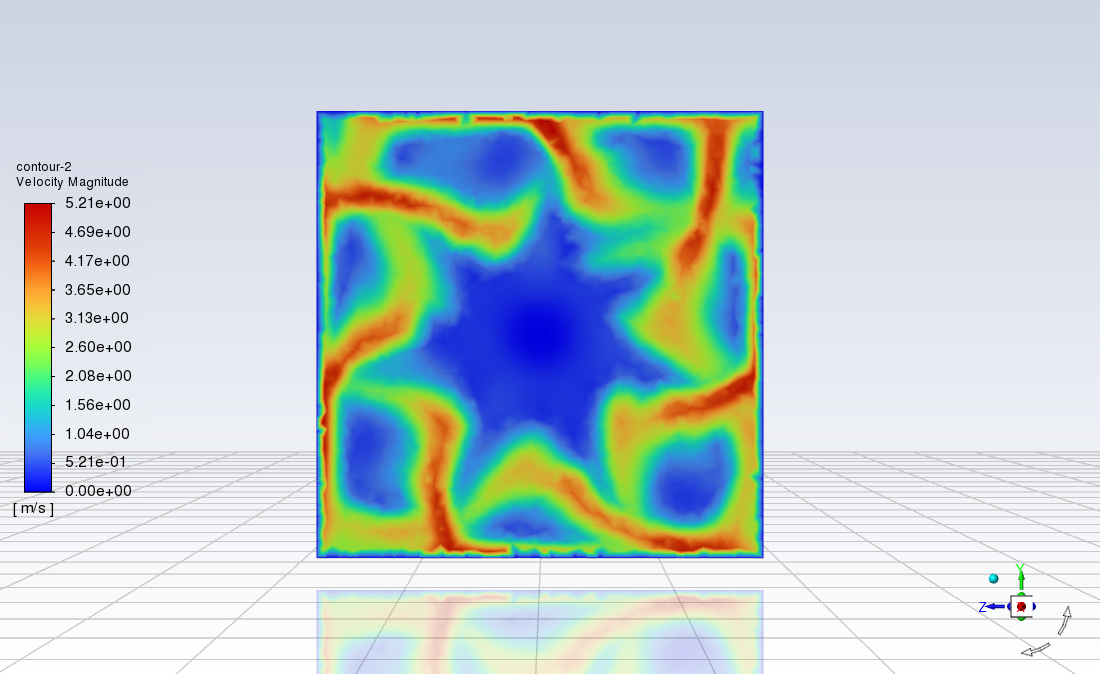
\includegraphics[width=0.6\linewidth]{dump/sal3.png}
            \caption{Mapa de velocidad en la salida para 4200 RPM.}
        \end{figure}
    \end{block}
\end{frame}

%% ====================== CONCLUSIONES =====================
\section{Conclusiones}

\begin{frame}{Conclusiones principales}
    \begin{itemize}
      \item El prototipo a escala y el modelo CFD muestran buena concordancia.
      \item La plataforma de adquisición basada en Arduino permite monitoreo en tiempo real de variables clave.
      \item Se estableció una línea base necesaria para entrenar futuros modelos de \emph{machine learning} orientados a mantenimiento predictivo.
    \end{itemize}
\end{frame}

\begin{frame}{Trabajo futuro}
    \begin{itemize}
      \item Refinamiento del modelo CFD.
      \item Expansión de la instrumentación.
        \item Incorporación de técnicas de aprendizaje automático.
      \item Escalar el enfoque a ventiladores en faenas reales.
      \item Análisis técnico-económico.
    \end{itemize}
\end{frame}

%% ====================== AGRADECIMIENTOS & BIBLIO =====================
%\section*{Referencias}
%
%\begin{frame}[allowframebreaks]{Referencias}
%    \nocite{*}
%    \printbibliography
%\end{frame}